\documentclass[11pt,a4paper]{article}
\usepackage[margin=1in]{geometry}
\usepackage{tikz}
\usepackage{xcolor}
\usepackage{enumitem}
\usepackage{fontenc}
\usepackage[utf8]{inputenc}
\usepackage{hyperref}
\usepackage{fancyhdr}
\usepackage{titlesec}
\usepackage{tabularx}
\usepackage{booktabs}
\usepackage{multicol}

\usetikzlibrary{shapes.geometric, arrows.meta, positioning, fit, calc, backgrounds, decorations.pathreplacing}

% Brand Colors
\definecolor{carone-orange}{RGB}{244,115,33}
\definecolor{carone-green}{RGB}{0,80,48}
\definecolor{carone-dark}{RGB}{18,42,38}
\definecolor{lightgray}{RGB}{245,245,245}
\definecolor{midgray}{RGB}{200,200,200}

% Styling
\hypersetup{colorlinks=true, linkcolor=carone-green, urlcolor=carone-orange}
\titleformat{\section}{\Large\bfseries\color{carone-dark}}{}{0em}{}[\titlerule]
\titleformat{\subsection}{\large\bfseries\color{carone-green}}{}{0em}{}

\pagestyle{fancy}
\fancyhf{}
\fancyhead[L]{\textcolor{carone-dark}{\textbf{Carone Labs}}}
\fancyhead[R]{\textcolor{carone-orange}{Website Architecture}}
\fancyfoot[C]{\thepage}
\renewcommand{\headrulewidth}{2pt}
\renewcommand{\headrule}{\hbox to\headwidth{\color{carone-orange}\leaders\hrule height \headrulewidth\hfill}}

\begin{document}

% Title Page
\begin{titlepage}
\centering
\vspace*{2cm}
{\Huge\bfseries\textcolor{carone-dark}{Carone Labs Website}\par}
\vspace{0.5cm}
{\LARGE\textcolor{carone-orange}{Architecture Document}\par}
\vspace{1.5cm}
{\large\textcolor{carone-green}{Next.js 14 $\cdot$ React 18 $\cdot$ TypeScript 5.4 $\cdot$ Tailwind CSS 3.4}\par}
\vspace{0.5cm}
{\large Deployed on Cloudflare Pages\par}
\vspace{2cm}


\begin{tikzpicture}
  \fill[carone-dark, rounded corners=8pt] (-4,-1.5) rectangle (4,1.5);
  \node[text=white, font=\Large\bfseries] at (0,0.4) {CARONE LABS};
  \node[text=carone-orange, font=\small] at (0,-0.4) {Innovative Solutions for Modern Challenges};
\end{tikzpicture}

\vfill
{\large Repository: \texttt{github.com/caronelabs/Website}\\[0.3cm]
Production: \texttt{website-6dw.pages.dev}\\[0.3cm]
Domain: \texttt{caronelabs.com}\par}
\vspace{1cm}
{\small Generated \today\par}
\end{titlepage}

\tableofcontents
\newpage

% ============================================================
\section{Technology Stack}
% ============================================================

\begin{center}
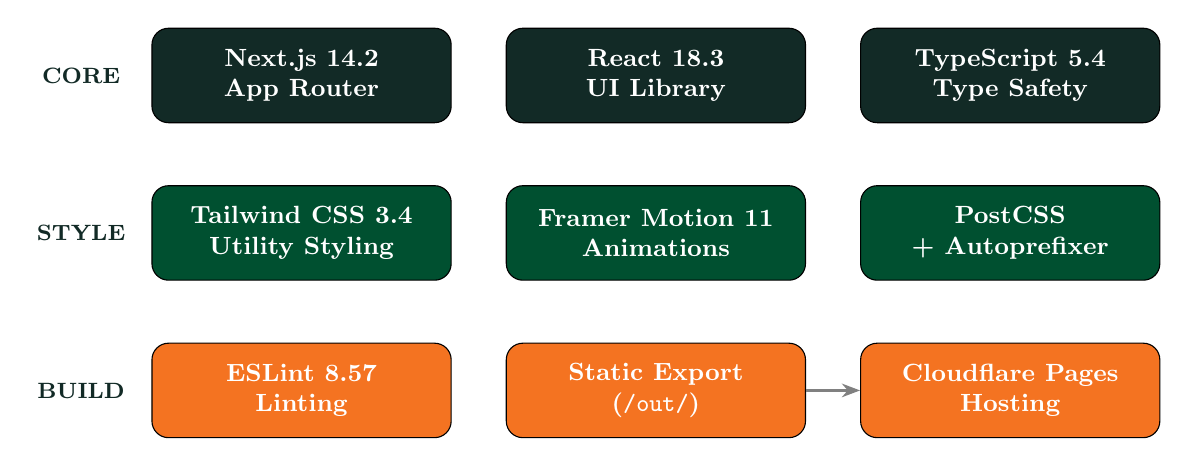
\begin{tikzpicture}[
  box/.style={draw, rounded corners=6pt, minimum width=3.8cm, minimum height=1.2cm, align=center, font=\small\bfseries},
]
  % Row 1 - Core
  \node[box, fill=carone-dark, text=white] (next) at (0,0) {Next.js 14.2\\App Router};
  \node[box, fill=carone-dark, text=white] (react) at (4.5,0) {React 18.3\\UI Library};
  \node[box, fill=carone-dark, text=white] (ts) at (9,0) {TypeScript 5.4\\Type Safety};

  % Row 2 - Styling & Animation
  \node[box, fill=carone-green, text=white] (tw) at (0,-2) {Tailwind CSS 3.4\\Utility Styling};
  \node[box, fill=carone-green, text=white] (fm) at (4.5,-2) {Framer Motion 11\\Animations};
  \node[box, fill=carone-green, text=white] (post) at (9,-2) {PostCSS\\+ Autoprefixer};

  % Row 3 - Tooling
  \node[box, fill=carone-orange, text=white] (eslint) at (0,-4) {ESLint 8.57\\Linting};
  \node[box, fill=carone-orange, text=white] (build) at (4.5,-4) {Static Export\\(\texttt{/out/})};
  \node[box, fill=carone-orange, text=white] (cf) at (9,-4) {Cloudflare Pages\\Hosting};

  % Labels
  \node[font=\footnotesize\bfseries, text=carone-dark] at (-2.8,0) {CORE};
  \node[font=\footnotesize\bfseries, text=carone-dark] at (-2.8,-2) {STYLE};
  \node[font=\footnotesize\bfseries, text=carone-dark] at (-2.8,-4) {BUILD};

  % Arrows
  \draw[-{Stealth}, thick, gray] (build) -- (cf);
\end{tikzpicture}
\end{center}

\subsection{Dependencies}

\begin{tabularx}{\textwidth}{llX}
\toprule
\textbf{Package} & \textbf{Version} & \textbf{Purpose} \\
\midrule
\texttt{next} & 14.2.0 & React framework with App Router, SSR/SSG \\
\texttt{react} & 18.3.0 & UI component library \\
\texttt{react-dom} & 18.3.0 & React DOM rendering \\
\texttt{framer-motion} & 11.0.0 & Declarative animations \\
\texttt{tailwindcss} & 3.4.0 & Utility-first CSS framework \\
\texttt{typescript} & 5.4.0 & Static type checking \\
\texttt{postcss} & 8.4.0 & CSS transformations \\
\texttt{autoprefixer} & --- & Vendor prefix automation \\
\texttt{eslint} & 8.57.0 & Code quality linting \\
\bottomrule
\end{tabularx}

\newpage

% ============================================================
\section{Deployment Pipeline}
% ============================================================

\begin{center}
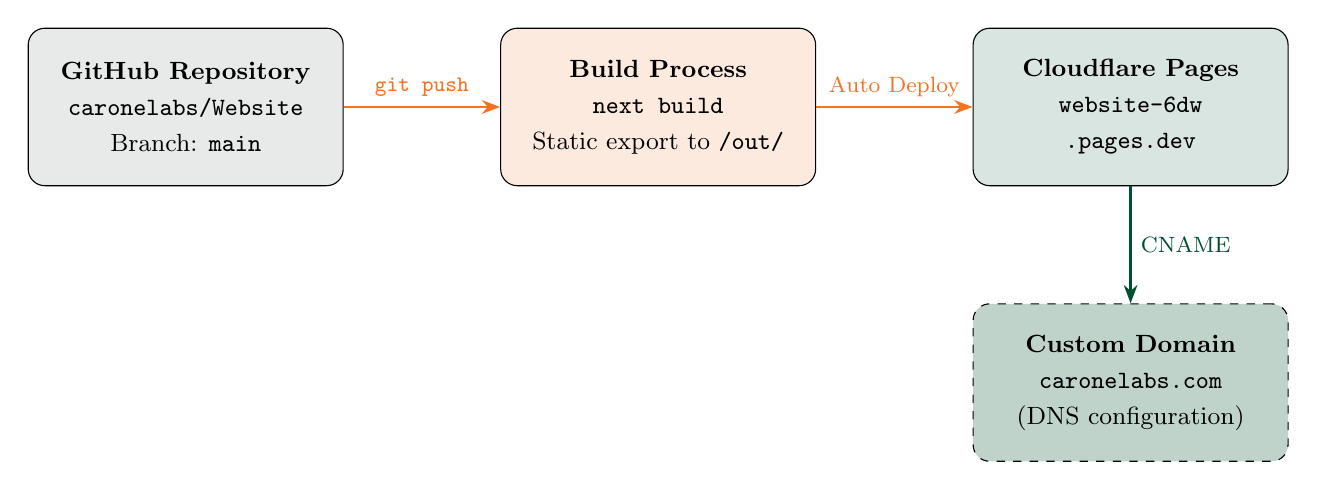
\begin{tikzpicture}[
  block/.style={draw, rounded corners=6pt, minimum width=4cm, minimum height=2cm, align=center, font=\small},
  arr/.style={-{Stealth}, thick, carone-orange},
]
  \node[block, fill=carone-dark!10] (repo) at (0,0) {\textbf{GitHub Repository}\\[2pt]\texttt{caronelabs/Website}\\[2pt]Branch: \texttt{main}};
  \node[block, fill=carone-orange!15] (build) at (6,0) {\textbf{Build Process}\\[2pt]\texttt{next build}\\[2pt]Static export to \texttt{/out/}};
  \node[block, fill=carone-green!15] (cf) at (12,0) {\textbf{Cloudflare Pages}\\[2pt]\texttt{website-6dw}\\[2pt]\texttt{.pages.dev}};
  \node[block, fill=carone-green!25, dashed] (domain) at (12,-3.5) {\textbf{Custom Domain}\\[2pt]\texttt{caronelabs.com}\\[2pt](DNS configuration)};

  \draw[arr] (repo) -- node[above, font=\footnotesize] {\texttt{git push}} (build);
  \draw[arr] (build) -- node[above, font=\footnotesize] {Auto Deploy} (cf);
  \draw[arr, carone-green] (cf) -- node[right, font=\footnotesize] {CNAME} (domain);
\end{tikzpicture}
\end{center}

\newpage

% ============================================================
\section{Project File Structure}
% ============================================================

\begin{center}
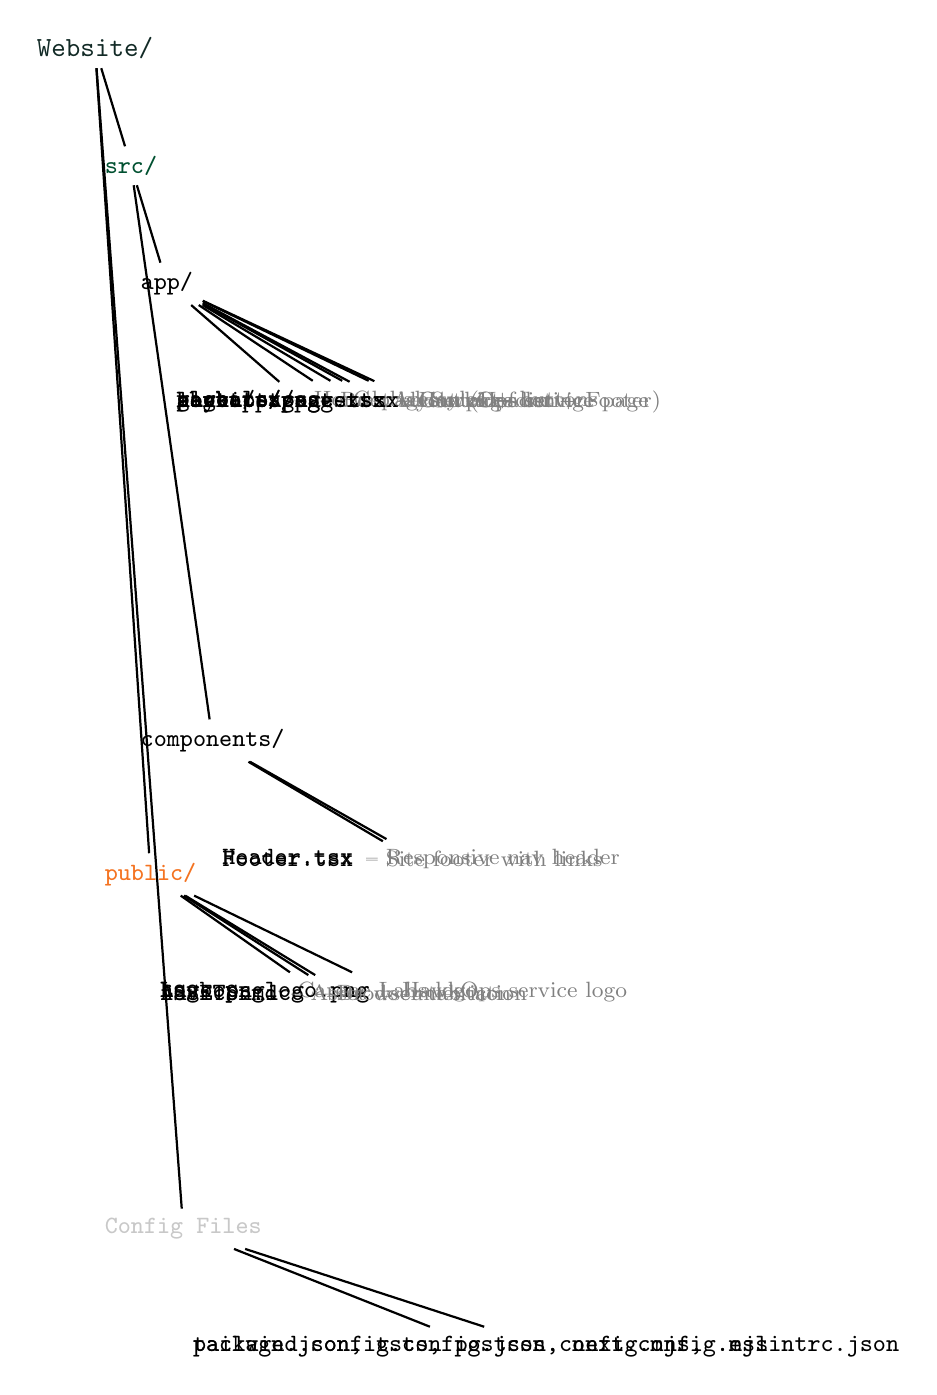
\begin{tikzpicture}[
  every node/.style={font=\ttfamily\small, anchor=west},
  level 1/.style={sibling distance=0cm, level distance=1.5cm},
]
  \node[font=\ttfamily\bfseries] {\textcolor{carone-dark}{Website/}}
    [grow=down, edge from parent/.style={draw, thick}]
    child { node {\textcolor{carone-green}{src/}}
      child { node {app/}
        child { node {layout.tsx \textcolor{gray}{\textrm{\footnotesize-- Root layout (Header + Footer)}}}}
        child { node {page.tsx \textcolor{gray}{\textrm{\footnotesize-- Home page}}}}
        child { node {globals.css \textcolor{gray}{\textrm{\footnotesize-- Global styles + buttons}}}}
        child { node {about/page.tsx \textcolor{gray}{\textrm{\footnotesize-- About page}}}}
        child { node {services/page.tsx \textcolor{gray}{\textrm{\footnotesize-- Services listing}}}}
        child { node {contact/page.tsx \textcolor{gray}{\textrm{\footnotesize-- Contact form}}}}
        child { node {hawkops/page.tsx \textcolor{gray}{\textrm{\footnotesize-- HawkOps service page}}}}
      }
      child { node[yshift=-5.8cm] {components/}
        child { node {Header.tsx \textcolor{gray}{\textrm{\footnotesize-- Responsive nav header}}}}
        child { node {Footer.tsx \textcolor{gray}{\textrm{\footnotesize-- Site footer with links}}}}
      }
    }
    child { node[yshift=-9cm] {\textcolor{carone-orange}{public/}}
      child { node {Logo.png \textcolor{gray}{\textrm{\footnotesize-- Carone Labs logo}}}}
      child { node {hawkops-logo.png \textcolor{gray}{\textrm{\footnotesize-- HawkOps service logo}}}}
      child { node {favicon.ico \textcolor{gray}{\textrm{\footnotesize-- Browser tab icon}}}}
      child { node {ASSETS.md \textcolor{gray}{\textrm{\footnotesize-- Asset documentation}}}}
    }
    child { node[yshift=-13.5cm] {\textcolor{midgray}{Config Files}}
      child { node {package.json, tsconfig.json, next.config.mjs}}
      child { node {tailwind.config.ts, postcss.config.mjs, .eslintrc.json}}
    };
\end{tikzpicture}
\end{center}

\newpage

% ============================================================
\section{Application Layout Architecture}
% ============================================================

\begin{center}
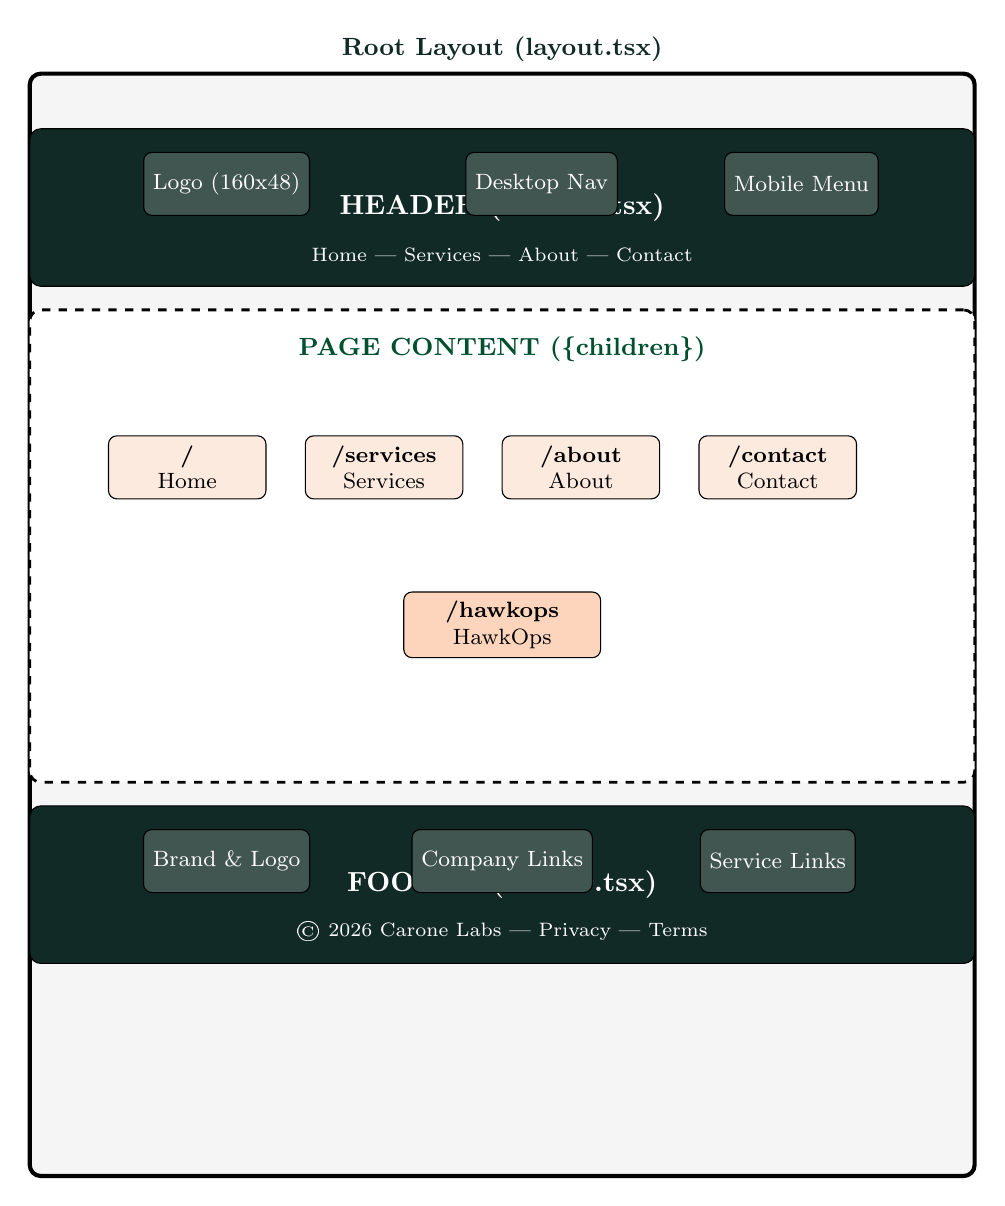
\begin{tikzpicture}[
  comp/.style={draw, rounded corners=4pt, minimum width=12cm, align=center, font=\small},
  inner/.style={draw, rounded corners=3pt, minimum height=0.8cm, align=center, font=\footnotesize},
]
  % Outer frame
  \node[comp, minimum height=14cm, fill=lightgray, line width=1.5pt, label={[font=\bfseries\small]above:\textcolor{carone-dark}{Root Layout (layout.tsx)}}] (layout) at (0,0) {};

  % Header
  \node[comp, fill=carone-dark, text=white, minimum height=2cm, font=\bfseries] (header) at (0,5.3) {HEADER (Header.tsx)};
  \node[inner, fill=carone-dark!80, text=white] at (-3.5,5.6) {Logo (160x48)};
  \node[inner, fill=carone-dark!80, text=white] at (0.5,5.6) {Desktop Nav};
  \node[inner, fill=carone-dark!80, text=white] at (3.8,5.6) {Mobile Menu};
  \node[font=\scriptsize, text=white] at (0,4.7) {Home | Services | About | Contact};

  % Page Content
  \node[comp, fill=white, minimum height=6cm, line width=1pt, dashed] (content) at (0,1) {};
  \node[font=\bfseries\small, text=carone-green] at (0,3.5) {PAGE CONTENT (\{children\})};

  % Route boxes inside content
  \node[inner, fill=carone-orange!15, minimum width=2cm] at (-4,2) {\textbf{/}\\Home};
  \node[inner, fill=carone-orange!15, minimum width=2cm] at (-1.5,2) {\textbf{/services}\\Services};
  \node[inner, fill=carone-orange!15, minimum width=2cm] at (1,2) {\textbf{/about}\\About};
  \node[inner, fill=carone-orange!15, minimum width=2cm] at (3.5,2) {\textbf{/contact}\\Contact};
  \node[inner, fill=carone-orange!30, minimum width=2.5cm] at (0,0) {\textbf{/hawkops}\\HawkOps};

  % Footer
  \node[comp, fill=carone-dark, text=white, minimum height=2cm, font=\bfseries] (footer) at (0,-3.3) {FOOTER (Footer.tsx)};
  \node[inner, fill=carone-dark!80, text=white] at (-3.5,-3) {Brand \& Logo};
  \node[inner, fill=carone-dark!80, text=white] at (0,-3) {Company Links};
  \node[inner, fill=carone-dark!80, text=white] at (3.5,-3) {Service Links};
  \node[font=\scriptsize, text=white] at (0,-3.9) {\copyright\ 2026 Carone Labs | Privacy | Terms};
\end{tikzpicture}
\end{center}

\newpage

% ============================================================
\section{Page Route Map}
% ============================================================

\begin{center}
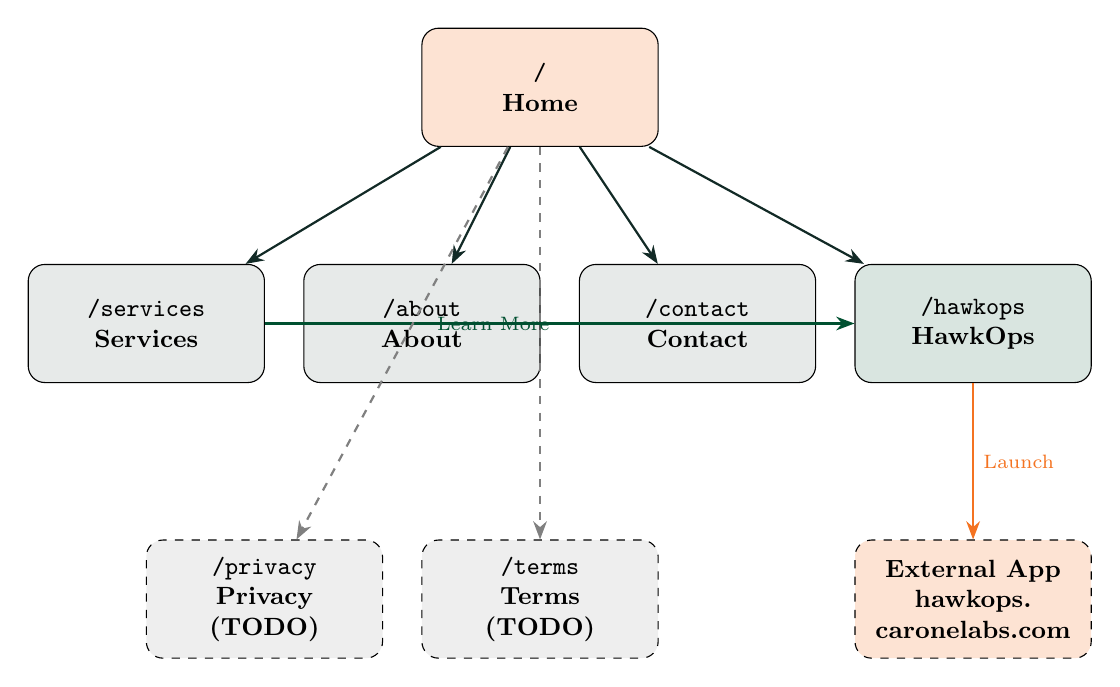
\begin{tikzpicture}[
  page/.style={draw, rounded corners=6pt, minimum width=3cm, minimum height=1.5cm, align=center, font=\small\bfseries, fill=carone-dark!10},
  ext/.style={draw, rounded corners=6pt, minimum width=3cm, minimum height=1.5cm, align=center, font=\small\bfseries, fill=carone-orange!20, dashed},
  arr/.style={-{Stealth}, thick},
]
  % Home
  \node[page, fill=carone-orange!20] (home) at (0,0) {\texttt{/}\\Home};

  % Level 2
  \node[page] (services) at (-5,-3) {\texttt{/services}\\Services};
  \node[page] (about) at (-1.5,-3) {\texttt{/about}\\About};
  \node[page] (contact) at (2,-3) {\texttt{/contact}\\Contact};
  \node[page, fill=carone-green!15] (hawkops) at (5.5,-3) {\texttt{/hawkops}\\HawkOps};

  % External
  \node[ext] (app) at (5.5,-6.5) {External App\\hawkops.\\caronelabs.com};

  % Future pages
  \node[page, fill=midgray!30, dashed] (privacy) at (-3.5,-6.5) {\texttt{/privacy}\\Privacy\\(TODO)};
  \node[page, fill=midgray!30, dashed] (terms) at (0,-6.5) {\texttt{/terms}\\Terms\\(TODO)};

  % Arrows from home
  \draw[arr, carone-dark] (home) -- (services);
  \draw[arr, carone-dark] (home) -- (about);
  \draw[arr, carone-dark] (home) -- (contact);
  \draw[arr, carone-dark] (home) -- (hawkops);

  % Services to hawkops
  \draw[arr, carone-green] (services) -- node[left, font=\scriptsize] {Learn More} (hawkops);

  % Hawkops to external
  \draw[arr, carone-orange] (hawkops) -- node[right, font=\scriptsize] {Launch} (app);

  % Footer links
  \draw[arr, gray, dashed] (home) -- (privacy);
  \draw[arr, gray, dashed] (home) -- (terms);
\end{tikzpicture}
\end{center}

\newpage

% ============================================================
\section{Home Page Layout}
% ============================================================

\begin{center}
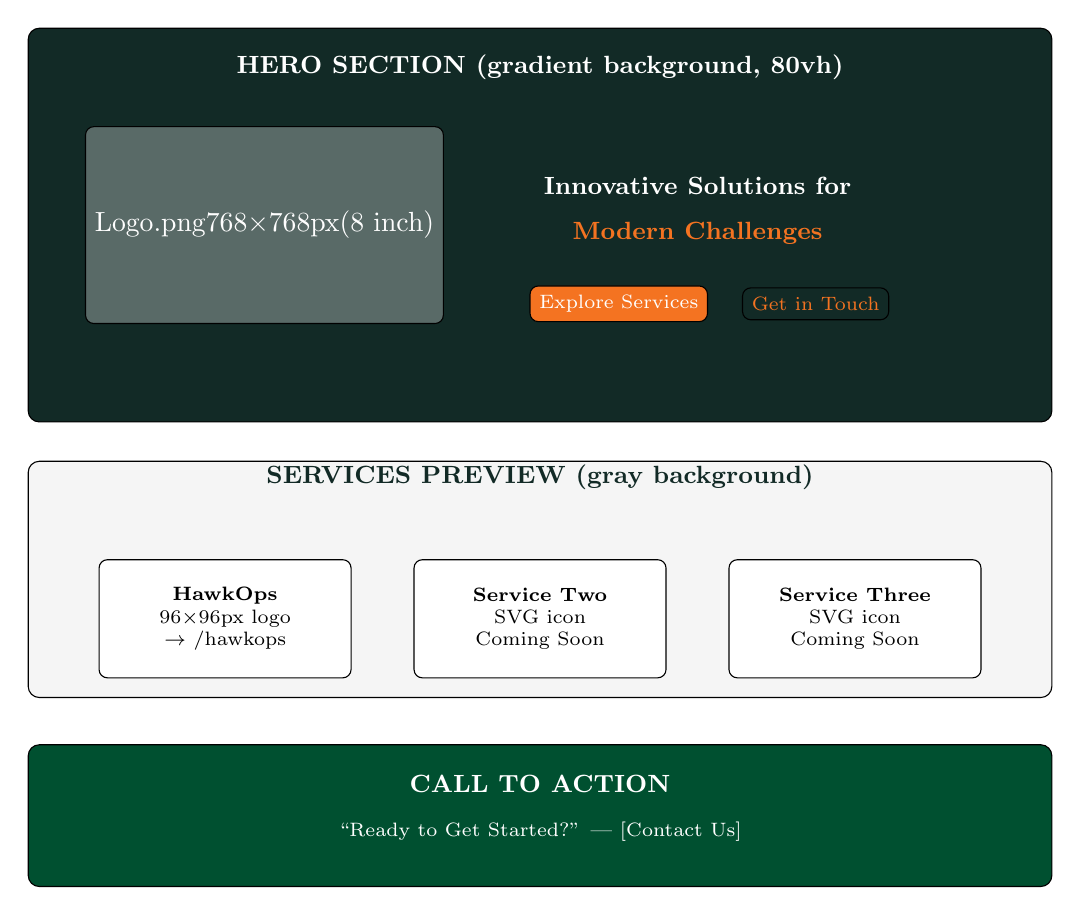
\begin{tikzpicture}[
  section/.style={draw, rounded corners=4pt, minimum width=13cm, align=center, font=\small},
]
  % Hero
  \node[section, fill=carone-dark, text=white, minimum height=5cm] (hero) at (0,0) {};
  \node[font=\bfseries\small, text=white] at (0,2) {HERO SECTION (gradient background, 80vh)};

  % Logo box
  \node[draw, fill=carone-dark!70, text=white, rounded corners=3pt, minimum width=3cm, minimum height=2.5cm] at (-3.5,0) {Logo.png\\768$\times$768px\\(8 inch)};

  % Text
  \node[text=white, font=\small, align=left] at (2,0.5) {\textbf{Innovative Solutions for}};
  \node[text=carone-orange, font=\small\bfseries] at (2,-0.1) {Modern Challenges};
  \node[draw, fill=carone-orange, text=white, rounded corners=3pt, font=\scriptsize] at (1,-1) {Explore Services};
  \node[draw, fill=none, text=carone-orange, rounded corners=3pt, font=\scriptsize] at (3.5,-1) {Get in Touch};

  % Services Preview
  \node[section, fill=lightgray, minimum height=3cm] (svc) at (0,-4.5) {};
  \node[font=\bfseries\small, text=carone-dark] at (0,-3.2) {SERVICES PREVIEW (gray background)};

  \node[draw, fill=white, rounded corners=3pt, minimum width=3.2cm, minimum height=1.5cm, align=center, font=\scriptsize] at (-4,-5) {\textbf{HawkOps}\\96$\times$96px logo\\$\rightarrow$ /hawkops};
  \node[draw, fill=white, rounded corners=3pt, minimum width=3.2cm, minimum height=1.5cm, align=center, font=\scriptsize] at (0,-5) {\textbf{Service Two}\\SVG icon\\Coming Soon};
  \node[draw, fill=white, rounded corners=3pt, minimum width=3.2cm, minimum height=1.5cm, align=center, font=\scriptsize] at (4,-5) {\textbf{Service Three}\\SVG icon\\Coming Soon};

  % CTA
  \node[section, fill=carone-green, text=white, minimum height=1.8cm] (cta) at (0,-7.5) {};
  \node[font=\bfseries\small, text=white] at (0,-7.1) {CALL TO ACTION};
  \node[font=\scriptsize, text=white] at (0,-7.7) {``Ready to Get Started?'' --- [Contact Us]};
\end{tikzpicture}
\end{center}

\newpage

% ============================================================
\section{HawkOps Page Layout}
% ============================================================

\begin{center}
\begin{tikzpicture}[
  section/.style={draw, rounded corners=4pt, minimum width=12cm, align=center, font=\small},
]
  % Hero
  \node[section, fill=carone-dark, text=white, minimum height=6cm] (hero) at (0,0) {};
  \node[font=\bfseries\small, text=white] at (0,2.5) {HERO SECTION (dark background)};

  \node[draw, fill=carone-dark!70, text=white, rounded corners=3pt, minimum width=3.5cm, minimum height=2.5cm] at (0,0.3) {hawkops-logo.png\\576$\times$576px\\(6 inch)};

  \node[font=\bfseries, text=white] at (0,-1.5) {HawkOps};
  \node[font=\scriptsize, text=gray!60] at (0,-2) {An immersive ITSM business simulation};

  % Content Card
  \node[section, fill=white, minimum height=4.5cm, drop shadow] (card) at (0,-5.5) {};
  \node[font=\bfseries\small, text=carone-dark] at (-3,-3.7) {About HawkOps};
  \node[draw, fill=green!10, text=green!50!black, rounded corners=3pt, font=\scriptsize] at (0.5,-3.7) {Available};

  \node[font=\scriptsize, text=gray, align=left] at (-2.5,-4.7) {%
    \textcolor{carone-orange}{\checkmark} Real-time IT service management\\
    \textcolor{carone-orange}{\checkmark} AI-powered incident management\\
    \textcolor{carone-orange}{\checkmark} Team collaboration features\\
    \textcolor{carone-orange}{\checkmark} Business simulation for UW-Whitewater
  };

  \node[draw, fill=carone-orange, text=white, rounded corners=3pt, font=\scriptsize\bfseries, minimum width=2.5cm] at (3.5,-5) {Launch HawkOps $\rightarrow$};
  \node[font=\tiny, text=gray] at (3.5,-5.7) {hawkops.caronelabs.com};
\end{tikzpicture}
\end{center}

\newpage

% ============================================================
\section{Brand \& Styling System}
% ============================================================

\subsection{Color Palette}

\begin{center}
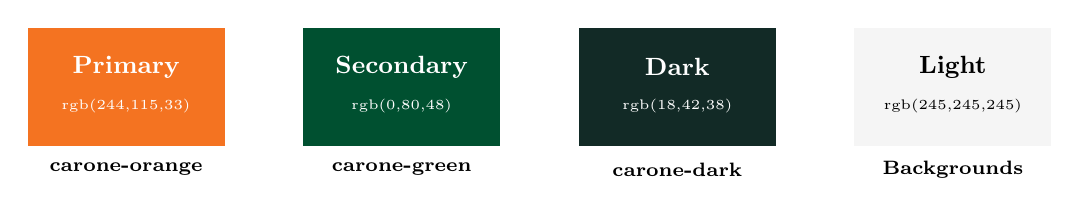
\begin{tikzpicture}
  % Color swatches
  \fill[carone-orange] (0,0) rectangle (2.5,1.5);
  \node[font=\small\bfseries, text=white] at (1.25,1) {Primary};
  \node[font=\tiny, text=white] at (1.25,0.5) {rgb(244,115,33)};
  \node[font=\scriptsize\bfseries] at (1.25,-0.3) {carone-orange};

  \fill[carone-green] (3.5,0) rectangle (6,1.5);
  \node[font=\small\bfseries, text=white] at (4.75,1) {Secondary};
  \node[font=\tiny, text=white] at (4.75,0.5) {rgb(0,80,48)};
  \node[font=\scriptsize\bfseries] at (4.75,-0.3) {carone-green};

  \fill[carone-dark] (7,0) rectangle (9.5,1.5);
  \node[font=\small\bfseries, text=white] at (8.25,1) {Dark};
  \node[font=\tiny, text=white] at (8.25,0.5) {rgb(18,42,38)};
  \node[font=\scriptsize\bfseries] at (8.25,-0.3) {carone-dark};

  \fill[lightgray] (10.5,0) rectangle (13,1.5);
  \node[font=\small\bfseries] at (11.75,1) {Light};
  \node[font=\tiny] at (11.75,0.5) {rgb(245,245,245)};
  \node[font=\scriptsize\bfseries] at (11.75,-0.3) {Backgrounds};
\end{tikzpicture}
\end{center}

\subsection{Button Components}

\begin{center}
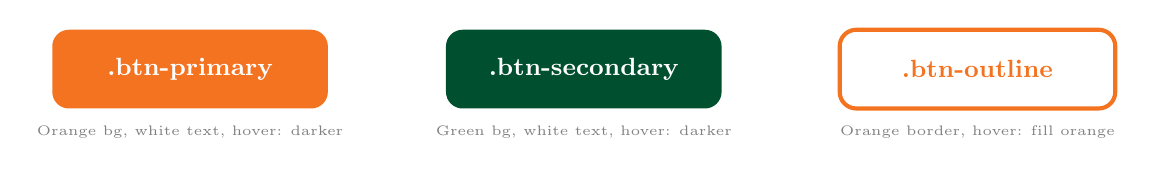
\begin{tikzpicture}
  % btn-primary
  \node[draw=none, fill=carone-orange, text=white, rounded corners=6pt, minimum width=3.5cm, minimum height=1cm, font=\small\bfseries] at (0,0) {.btn-primary};
  \node[font=\tiny, text=gray] at (0,-0.8) {Orange bg, white text, hover: darker};

  % btn-secondary
  \node[draw=none, fill=carone-green, text=white, rounded corners=6pt, minimum width=3.5cm, minimum height=1cm, font=\small\bfseries] at (5,0) {.btn-secondary};
  \node[font=\tiny, text=gray] at (5,-0.8) {Green bg, white text, hover: darker};

  % btn-outline
  \node[draw=carone-orange, line width=1.5pt, fill=none, text=carone-orange, rounded corners=6pt, minimum width=3.5cm, minimum height=1cm, font=\small\bfseries] at (10,0) {.btn-outline};
  \node[font=\tiny, text=gray] at (10,-0.8) {Orange border, hover: fill orange};
\end{tikzpicture}
\end{center}

\subsection{Typography}

\begin{tabularx}{\textwidth}{lX}
\toprule
\textbf{Element} & \textbf{Style} \\
\midrule
Font Family & Inter (Google Fonts), system-ui fallback \\
Page Titles & \texttt{text-4xl md:text-5xl font-bold} \\
Hero Headings & \texttt{text-4xl md:text-6xl font-bold} \\
Section Headings & \texttt{text-2xl md:text-3xl font-bold} \\
Body Text & \texttt{text-lg text-gray-600} \\
\bottomrule
\end{tabularx}

\newpage

% ============================================================
\section{Component Dependency Map}
% ============================================================

\begin{center}
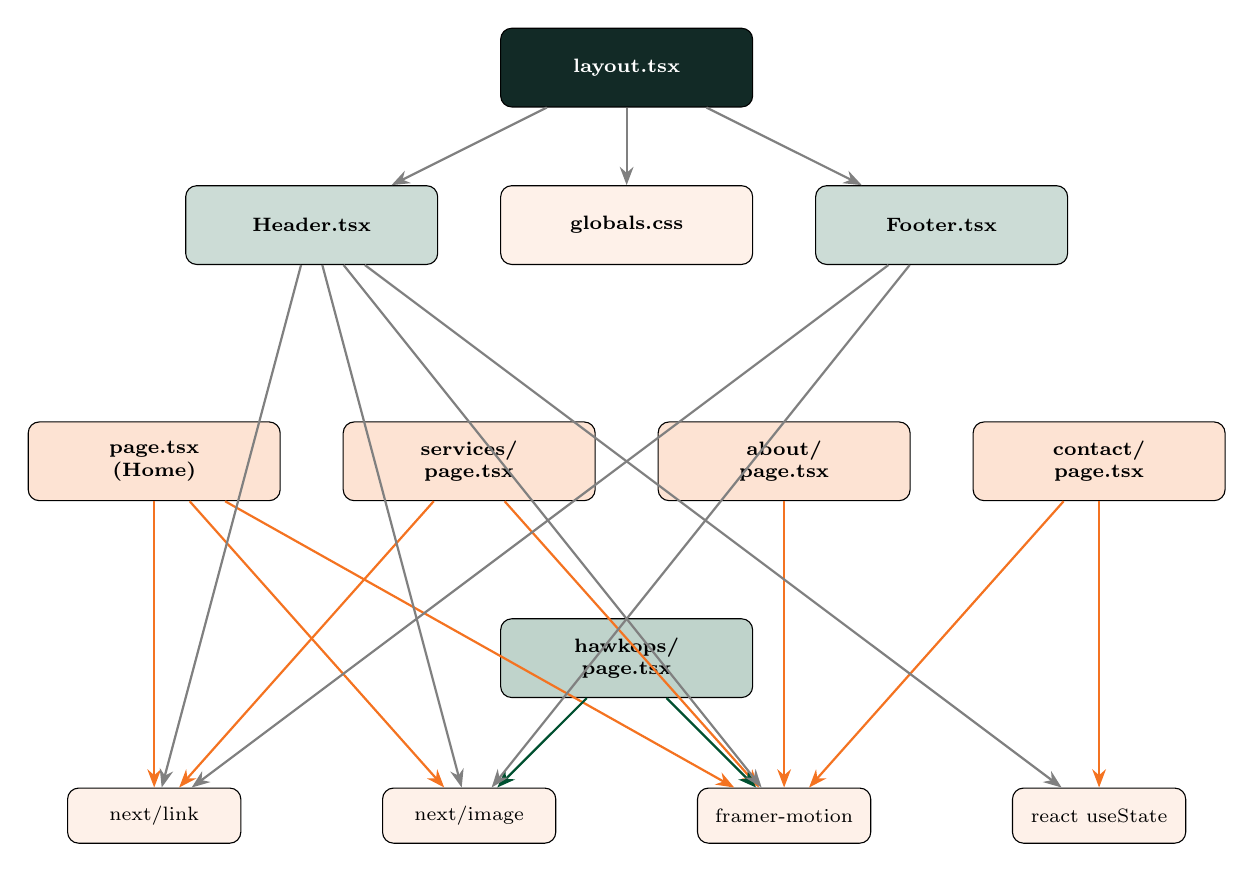
\begin{tikzpicture}[
  file/.style={draw, rounded corners=4pt, minimum width=3.2cm, minimum height=1cm, align=center, font=\scriptsize\bfseries},
  lib/.style={draw, rounded corners=4pt, minimum width=2.2cm, minimum height=0.7cm, align=center, font=\scriptsize, fill=carone-orange!10},
  dep/.style={-{Stealth}, thick, gray},
]
  % Layout
  \node[file, fill=carone-dark, text=white] (layout) at (0,0) {layout.tsx};
  \node[file, fill=carone-green!20] (header) at (-4,-2) {Header.tsx};
  \node[file, fill=carone-green!20] (footer) at (4,-2) {Footer.tsx};
  \node[file, fill=carone-orange!10] (css) at (0,-2) {globals.css};

  % Pages
  \node[file, fill=carone-orange!20] (home) at (-6,-5) {page.tsx\\(Home)};
  \node[file, fill=carone-orange!20] (svc) at (-2,-5) {services/\\page.tsx};
  \node[file, fill=carone-orange!20] (about) at (2,-5) {about/\\page.tsx};
  \node[file, fill=carone-orange!20] (contact) at (6,-5) {contact/\\page.tsx};
  \node[file, fill=carone-green!25] (hawk) at (0,-7.5) {hawkops/\\page.tsx};

  % Libraries
  \node[lib] (nextlink) at (-6,-9.5) {next/link};
  \node[lib] (nextimg) at (-2,-9.5) {next/image};
  \node[lib] (fm) at (2,-9.5) {framer-motion};
  \node[lib] (useState) at (6,-9.5) {react useState};

  % Layout deps
  \draw[dep] (layout) -- (header);
  \draw[dep] (layout) -- (footer);
  \draw[dep] (layout) -- (css);

  % Page deps
  \draw[dep, carone-orange] (home) -- (nextlink);
  \draw[dep, carone-orange] (home) -- (nextimg);
  \draw[dep, carone-orange] (home) -- (fm);

  \draw[dep, carone-orange] (svc) -- (nextlink);
  \draw[dep, carone-orange] (svc) -- (fm);

  \draw[dep, carone-orange] (about) -- (fm);

  \draw[dep, carone-orange] (contact) -- (fm);
  \draw[dep, carone-orange] (contact) -- (useState);

  \draw[dep, carone-green] (hawk) -- (nextimg);
  \draw[dep, carone-green] (hawk) -- (fm);

  \draw[dep] (header) -- (nextlink);
  \draw[dep] (header) -- (nextimg);
  \draw[dep] (header) -- (useState);
  \draw[dep] (header) -- (fm);

  \draw[dep] (footer) -- (nextlink);
  \draw[dep] (footer) -- (nextimg);
\end{tikzpicture}
\end{center}

\newpage

% ============================================================
\section{Asset Usage}
% ============================================================

\begin{center}
\begin{tabularx}{\textwidth}{llllX}
\toprule
\textbf{Asset} & \textbf{Used In} & \textbf{Display Size} & \textbf{Inches} & \textbf{Notes} \\
\midrule
Logo.png & Home page hero & 768$\times$768px & 8$\times$8 & Left side of hero \\
Logo.png & Header & 160$\times$48px & --- & Navigation bar \\
Logo.png & Footer & 160$\times$48px & --- & Footer brand \\
hawkops-logo.png & Home services & 96$\times$96px & 1$\times$1 & Service card icon \\
hawkops-logo.png & /hawkops page & 576$\times$576px & 6$\times$6 & Hero section, centered \\
favicon.ico & Browser tab & 16$\times$16px & --- & Tab icon \\
\bottomrule
\end{tabularx}
\end{center}

% ============================================================
\section{Animation System}
% ============================================================

All animations use \textbf{Framer Motion} with the following patterns:

\begin{tabularx}{\textwidth}{lllX}
\toprule
\textbf{Pattern} & \textbf{Trigger} & \textbf{Effect} & \textbf{Used In} \\
\midrule
\texttt{fadeInUp} & Page load / scroll & Opacity 0$\to$1, Y +20$\to$0 & Service cards, sections \\
\texttt{slideFromLeft} & Page load & Opacity 0$\to$1, X -30$\to$0 & Home page logo \\
\texttt{staggerChildren} & Scroll into view & 0.1s delay per child & Service grids \\
\texttt{scaleIn} & Scroll into view & Scale 0.95$\to$1 & CTA sections \\
\texttt{AnimatePresence} & State toggle & Height expand/collapse & Mobile menu \\
\bottomrule
\end{tabularx}

\vspace{0.5cm}
All scroll-triggered animations use \texttt{once: true} to fire only on first view.

\newpage

% ============================================================
\section{Implementation Status}
% ============================================================

\subsection{Completed}

\begin{itemize}[leftmargin=1.5cm]
  \item[\textcolor{carone-green}{\checkmark}] 5 pages: Home, Services, About, Contact, HawkOps
  \item[\textcolor{carone-green}{\checkmark}] Responsive navigation with mobile hamburger menu
  \item[\textcolor{carone-green}{\checkmark}] Brand color system (orange, green, dark)
  \item[\textcolor{carone-green}{\checkmark}] HawkOps service integration with dedicated page
  \item[\textcolor{carone-green}{\checkmark}] Framer Motion animations throughout
  \item[\textcolor{carone-green}{\checkmark}] Static export for Cloudflare Pages
  \item[\textcolor{carone-green}{\checkmark}] TypeScript type safety
  \item[\textcolor{carone-green}{\checkmark}] Contact form frontend
\end{itemize}

\subsection{TODO}

\begin{itemize}[leftmargin=1.5cm]
  \item[\textcolor{carone-orange}{$\circ$}] Contact form backend (Formspree / Cloudflare Workers / custom API)
  \item[\textcolor{carone-orange}{$\circ$}] Privacy Policy page (\texttt{/privacy})
  \item[\textcolor{carone-orange}{$\circ$}] Terms of Service page (\texttt{/terms})
  \item[\textcolor{carone-orange}{$\circ$}] Service Two implementation
  \item[\textcolor{carone-orange}{$\circ$}] Service Three implementation
  \item[\textcolor{carone-orange}{$\circ$}] DNS configuration: \texttt{caronelabs.com} $\to$ Cloudflare Pages
  \item[\textcolor{carone-orange}{$\circ$}] Social media preview image (\texttt{og-image.png})
\end{itemize}

\end{document}
